\documentclass[../report.tex]{subfiles}
\begin{document} \chapter{Method} This method chapter subjects the reader to the framework used to qualitatively compare the different algorithms on the given dataset.

\section{Method Design Overview}
In order to generate results and compare the three different SSC algorithms with k-means, a method design was planned and executed. The overall design is shown in \cref{fig:method}, it includes the step of \textit{Preprocessing}, \textit{Implementation}, \textit{Parameter Selection} and \textit{External Evaluation}.

\begin{figure}[h]
  \begin{center}
    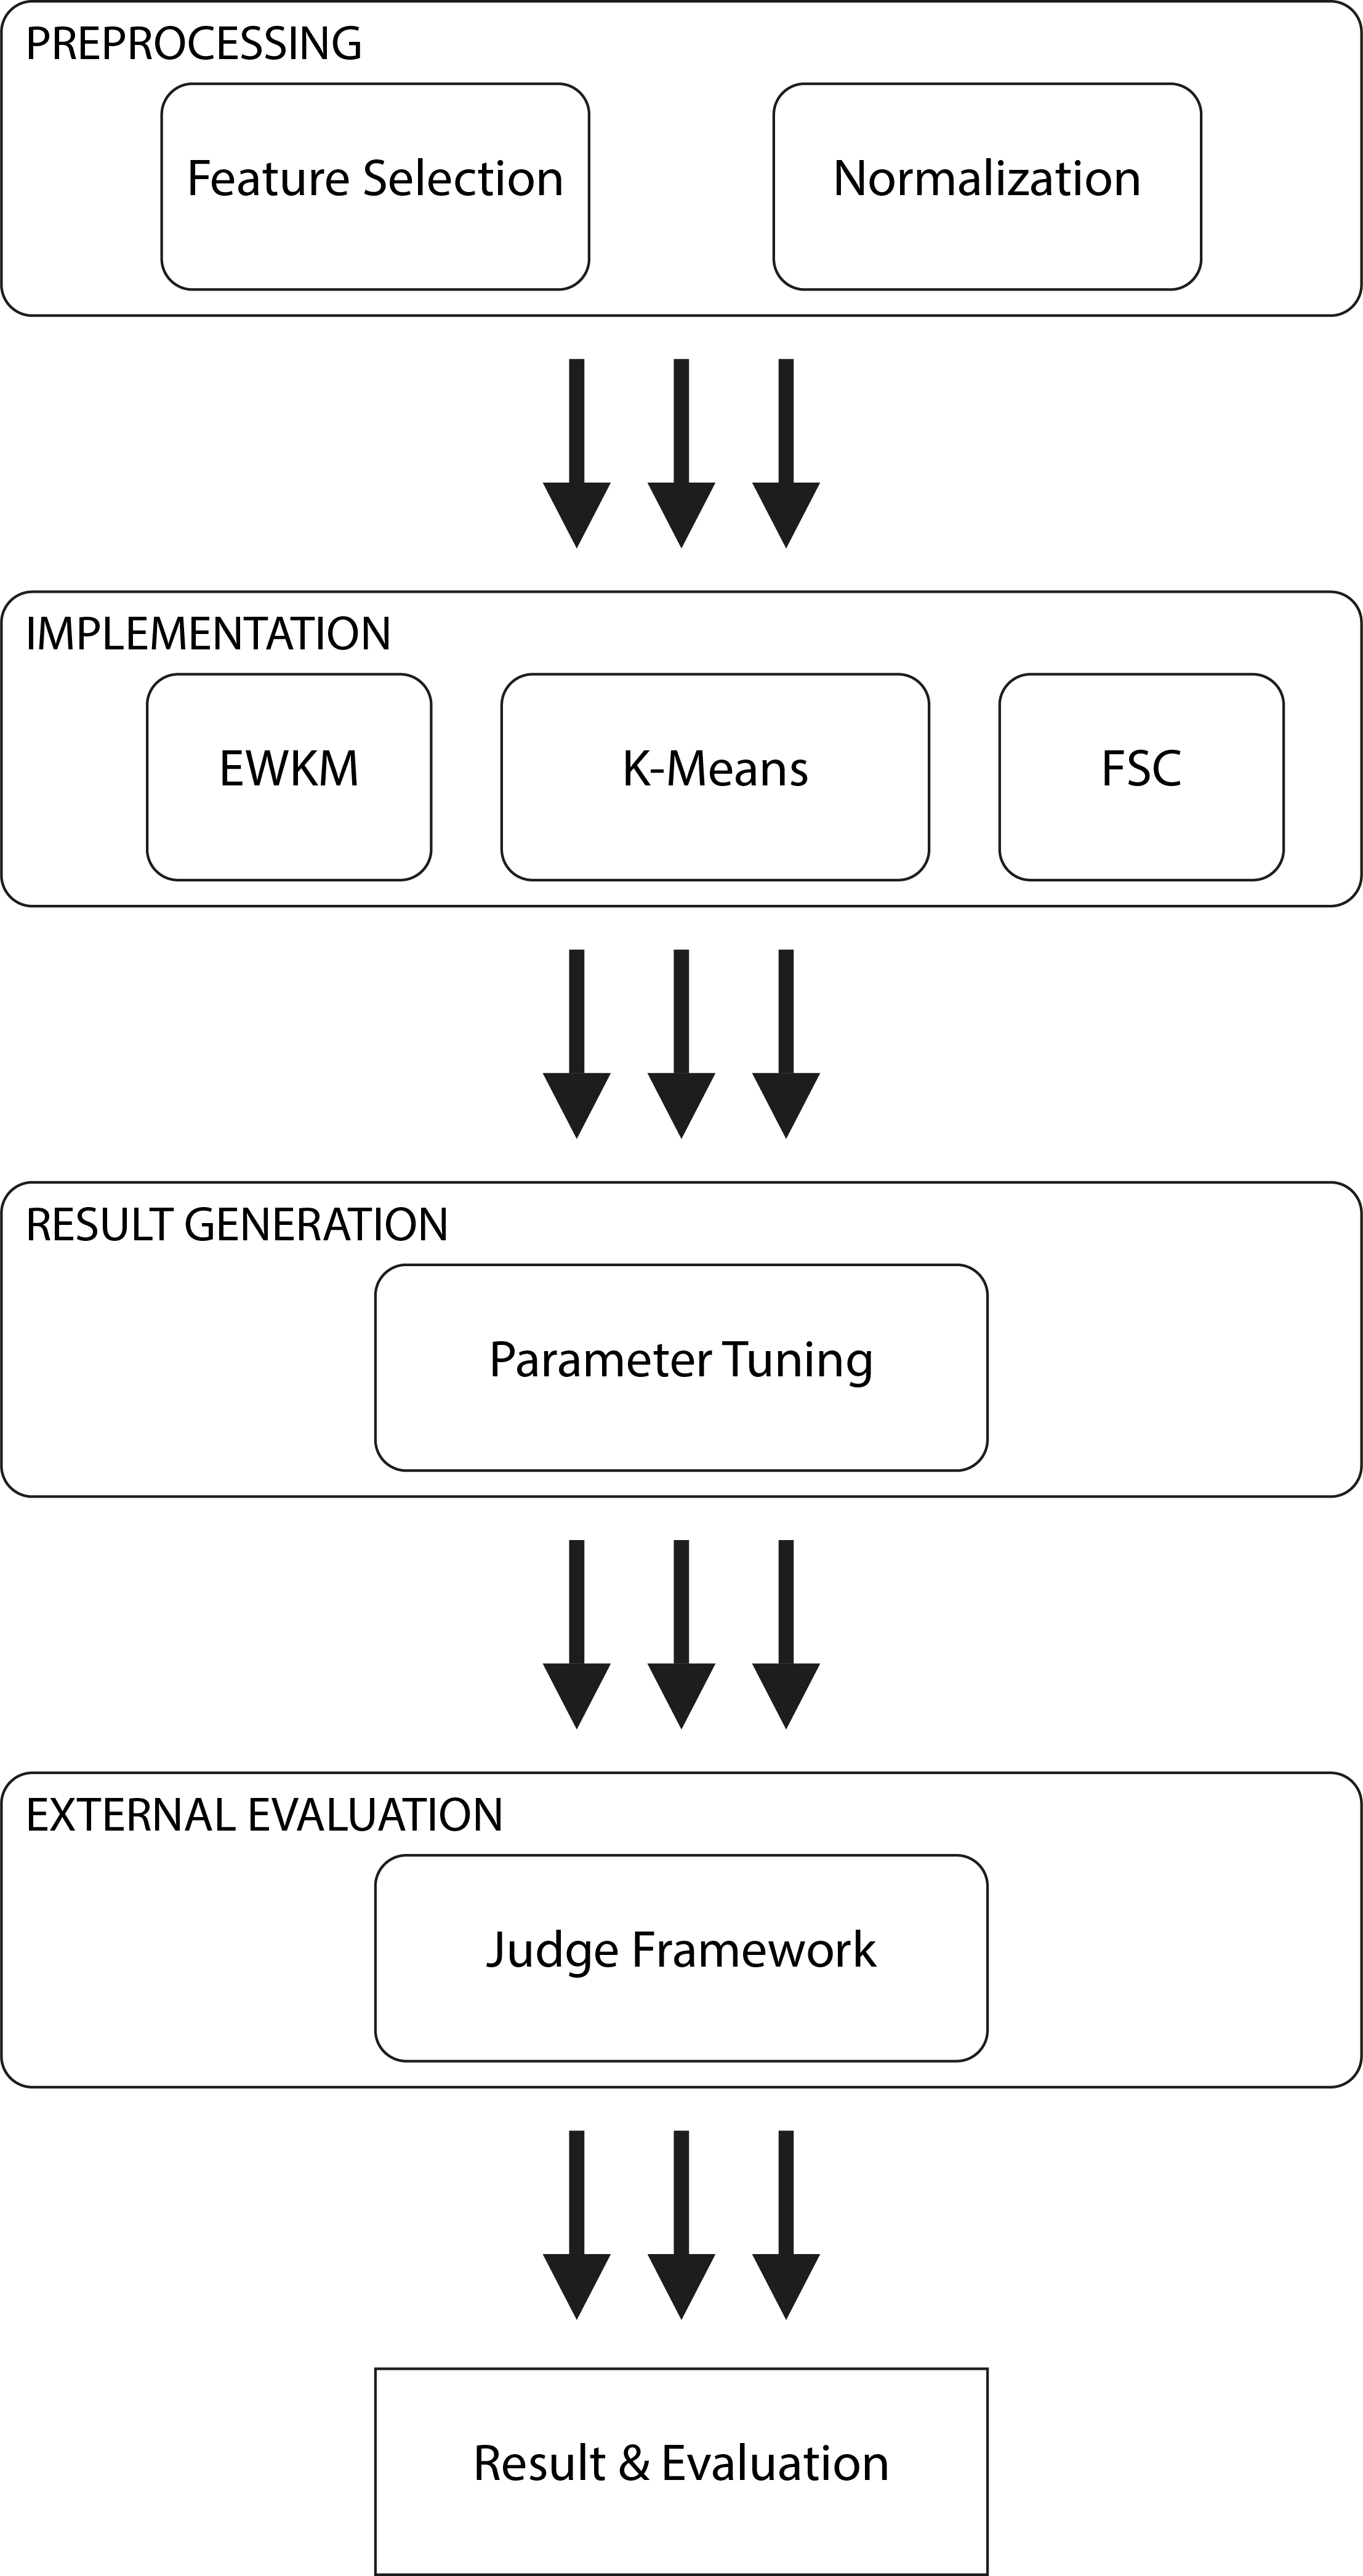
\includegraphics[width=0.4\textwidth]{Design}
  \end{center}
  \caption{Method Design}\label{fig:method}
\end{figure}
\section{Dataset}
\label{sec:dataset}
% Clustering analysis will be made on a real-world-, high-dimensional- and, mixed-dataset.
The given dataset is a real-world, high-dimensional mixed-dataset. It is a set of \textit{song objects} extracted from an internal music database. There are in total $5\cdot10^7$ songs in the dataset. Each song is a vector of features where different features describe the song through different song properties. The vector consists of two types of features, general metadata and audio-based features.

The general metadata includes attributes that predominantly identify the song independent of audio analysis. Features of the type includes \textit{Album} (string), \textit{Artist} (string), \textit{Title} (string) and \textit{Year of Origin} (ordinal). The type also includes \textit{BPM} (numerical, zero to around 200) and \textit{Energy-feel} (ordinal, one to ten). These features include both numerical and categorical features --- features stored as strings can be converted to categorical data.

The core features are the audio-based features, and are derived from a supervised neural network. They are a sample of the neuron weights in a network trained to determine the genre of a song. Each song consists of an audio embedding --- devised from an audio spectrogram --- and a \textit{genre} label --- used to train the network.

Our dataset includes the genre feature. There are $33$ possible genres for the songs in the dataset.






% For our dataset there is 


% So, the reason for defining the features as audio based is due to audio data used to train the network.


% They are a sample of the neural weights of a trained supervised neural network.

% The source of the features are a trained supervised neural network. The input of the network are audio embeddings of songs --- devised from an audio spectrogram --- that have a predetermined genre. The genre is utilized as a label to train the network for the task of classifying the genre of an audio embedding. In total there are $33$ different genres a song can be labeled as.


% They represent the song through its audio properties. There in


% They represent the song with features based on audio properties of a song. There are 160 of these features, together they can be seen as 160-dimensional vector where each dimension represents a feature.


% Audio features of our dataset are a representative sample of neuron weights in the trained supervised neural network. The genre label is also a feature that exist in a smaller subset of our given dataset.

% \begin{color}{red}{
% \subsection{MFCC}
% To understand MFCC we need to first understand how humans perceive sound and how speech is created. Humans are more sensitive to frequency differences at lower frequencies compared to higher frequencies. The Mel-scale takes the differences in sensitivity into account by creating a logarithmic scale. Human speech is generated by the shape of the vocal tract. The shape determines what sound is created.
% A power spectrum describes how much power is in the frequency component of a signal. The envelope of the power spectrum can be used to represent the shape of the vocal tract of the given audio. An MFCC represents the envelope \cite{Paliwal2010}. With the shape of the tract represented, generated phonemes can be determined of the vocals of the audio.
% }\end{color}


\section{Preprocessing}
The amount of dataset objects and features were reduced in the preprocessing stage for various reasons. For the ease of testing --- reducing computation time --- the original dataset of songs was sampled and reduced to a size of $5 \cdot 10^4$.

The thesis focuses on the problem of clustering high-dimensional data. Mixed-data SSC algorithms are not widely available online, and so the choice was to use the numerical clustering methods of EWKM, LEKM, FSC. This forced the exclusion of features that were not numerical. Given that the audio vector was used to categorize songs in the mentioned neural network, the hypothesis was that clustering analysis could also be done exclusively on that feature-space. The dataset was therefore preprocessed to only include the subspace of audio-features.

As a next step in preprocessing, features were normalized to the same variance --- a way to make sure that all features have the same impact on the algorithm. For normalization \textit{Z-score} was used, see \cref{eq:z-score}. $X_j$ is the vector of all datapoints for feature $j$, $\mu_j$ is the mean values for datapoints in feature $j$, $\sigma_{j}$ is the standard deviation of feature $j$ and $Z_j$ is the normalized vector.

\begin{equation}
  \label{eq:z-score}
  Z_j = \frac{X_j - \mu_j}{\sigma_j}
\end{equation}

\section{Implementation}

\subsection{EWKM}
An implementation of the EWKM algorithm is available in \textit{R} and \textit{CSRAN} through the \textit{wskm} package \cite{wskm2014hz}. The code is written in $C$ and wrapped for $R$. All of the source code is obtainable from Github\footnote{https://github.com/SimonYansenZhao/wskm/}.

There are modifications made in the implementation that differ from the original research paper \cite{Jing2007}. Additional normalization steps have been added when calculating $w_{lj}$. \Cref{eq:newlambda} shows how $w_{lj}$, the feature weight, is updated in the given implementation. Occurrences of empty clusters during partitioning are managed by re-sampling cluster centers, i.e. restarting the algorithm; in the original algorithm empty clusters were not treated. Finally, a convergence delta can be set by the user which decides the percentage of change needed between two iterations for convergence.

\begin{align}
  \lambda_{lj} &= \exp\bigg({\Big(\frac{-D_{lj}}{\gamma}\Big) - \max_{\forall{t} \in C_l}\Big({\frac{-D_{lt}}{\gamma}}\Big)}\bigg) \\
  \lambda_{lj} &= \max\bigg(\frac{\lambda_{lj}}{\sum_{t=1}^{m}{\lambda_{lt}}}, \frac{0.0001}{m}\bigg)\\
  \label{eq:newlambda}
  w_{lj} &= \frac{\lambda_{lj}}{\sum^{m}_{t=1}{\lambda_{ lt }}}
\end{align}

Per request of the stakeholder along with the author's familiarity with Python and Pandas DataFrame, the code was re-wrapped for Python using numpy-C-API \cite{numpy-c} --- allowing for the dataset to be sent in to the algorithm as a numpy array. The C-code was tweaked to not be dependent on R's \textit{unif\_rand() function}.

\subsection{FSC}
The FSC implementation was created by the thesis author and is based on the C-code of EWKM. The methods of calculating cost, updating weights and updating cluster memberships were modified to correspond to the FSC algorithm as shown in \cref{eq:cost-fsc}, and \cref{eq:fsc}. $\gamma$ is replaced by $\beta$, and the small value of $\epsilon$ was set to $0.001$ as proposed in \cite{Gan2006}.

\subsection{LEKM}
LEKM like \textit{FSC} was created by the author and based on the source code of EWKM \cite{wskm2014hz}. The same steps are necessary for this algorithm as EWKM, since both are based on the negative entropy. The difference is the addition of logarithmic distances in when updating the centers, partitions, and feature weights. How they were updated correspond to the equations of LEKM shown in \crefrange{eq:lekm}{eq:lekm2}.

A slight difference is that the right-hand side, i.e. the negative entropy is dropped from when updating partitions. The modification is based on a discussion with one of the authors of the original \textit{LEKM} paper. The gist of the discussion was that the entropy should not be used for updating clusters, and could result in negative distances.

\subsection{K-means}
EWKM is equivalent to K-means when $\lim_{\gamma \to 0}$ although simply setting $\gamma = 0$ forces division by zero. For this reason K-means needs its own implementation.

K-means is available for Python thorough various packages such as PyClustering \cite{Novikov2019}. However, to allow a fair comparison between algorithms, K-means was re-implemented by the author in \textit{C} based on the EWKM source code.

% All algorithm specific parameters were ran with all $k$ candidates. The best performing combination of parameters are deemed the best candidates for the algorithm.
\section{Parameter Selection}
% The sections below describe how the parameters of the different algorithms were chosen.
Algorithms were tested with multiple candidate parameters on the dataset in order to find the most suitable parameters. The impact of the different parameters was compared through an external validation index, a \textit{purity} score. The best parameters in accordance to the index were deemed the most suitable, and chosen as the parameters for the algorithm for further tests.

For generating results, convergence was set to occur if the cost delta between previous iteration and current was less than $0.5\%$.

\subsection{Purity}
An external validation index was created using the \textit{genre} feature as a ground truth in combination with the measurement of purity. To create the purity score, the most dominant genre of each cluster was aggregated and divided by the total amount of songs in the dataset.

\subsection{Amount of Clusters}
The problem of deciding the amount of clusters ($k$) is global as all the clustering algorithms chosen are partition based. This section describes how $k$ was chosen for all of the chosen algorithms.

For the choice of $k$, it was decided to not use a competitive learning strategy. The strategy would add another layer of complexity on the algorithms and a possible point of error. $k$ was instead based on the \textit{purity} results of the whole sample.

% The amount of clusters i.e. $k$, could have been decided on a smaller sample of the dataset, or through the use of a competitive learning strategy as discussed in the background. Due to the already relative small sample of the whole dataset and an algorithm that is linear in time, $k$ was based on the results of the whole sample dataset with respect to the best $\gamma$ in regards to the cost function.

Candidate values of $k$ were restricted to $50$, $100$, and $500$ in order to reduce the time needed to generate results. The values were chosen to give an approximation on how large \textit{k} should be. The minimum of $50$ clusters was based on that the number of genres in the dataset was $33$, and generated clusters should at least be as specific as a genre label. $500$ was decided as the maximum amount for $k$ to keep the average cluster size to be above $100$.

% For the later external evaluation stage with composers, $k$ was picked based on the overall best purity score of the algorithms.

% Relying on this criteria to evaluate the results had some downsides. A good song cluster does not have to be genre homogenic. A good cluster could hypothetically have been Christmas music and hold multiple genres. According to purity, this would be a bad cluster.

% The decision was still made to use purity for parameter tuning. While it does have its' downsides, the belief is that a higher purity score should in general indicate higher average cluster quality.

% To not disregard the problems with purity another external evaluation was made with the best performing SSC algorithm and K-means through the usage of judges. The evaluation is described in the next subchapter.

\subsection{EWKM}
EWKM introduces the $\gamma$ parameter. The recommended range of $\gamma \approx (0.5, 3)$ which was mentioned in \citeauthor{Jing2007} \cite{Jing2007} and \citeauthor{wskm2014hz} \cite{wskm2014hz}, was extended with smaller values $(0.0005,$ $0.001,$ $0.005,$ $0.01,$ $0.05,$ $0.1)$ as candidate values. The smaller values were added to avoid possible problems with the objective function being negative due to a large negative entropy.

Results of gamma values with immediate convergence were discarded as the behaviour was deemed undesirable, and not what was expected from the algorithms.

\subsection{FSC}
The unique parameters of \textit{FSC}, $\beta$ --- the fuzziness variable, and $\epsilon$ --- a small constant, were set to $2.1$ and $0.00001$, respectively, in \cite{Gan2006}. In our tests $\beta$ was varied between $1.5$ and $30$ while $\epsilon$ was kept to the value mentioned in the report \citeauthor{Gan2006} \cite{Gan2006}.

\subsection{LEKM}
In \citeauthor{Gan2016} \cite{Gan2016} values of $\beta$ were varied between $1$ and $16$ with a decreasing score after a value of $2.0$. Our candidate values ranged between $0.5$ and $10$. Similarly to EWKM, results of immediate convergence were disregarded.

% \begin{color}{red}
% $\gamma$ is a hyper-parameter of EWKM and LEKM. In short, $\gamma$ determines the likeliness to cluster on more or less features. For any given dataset the ideal $\gamma$ can vary. An ideal $\gamma$ is found (in this scenario) when there is no other $\gamma$ value that can result in a better purity.
% \end{color}

% $\gamma$ was chosen by iteratively testing different values of the parameter as an input for the algorithms, from small ($1 * 10^{-3}$) to large ($\gamma = 3$). The best $\gamma$ was chosen based on purity and, if values showed similar results the smallest value was chosen.

\subsection{K-means}
K-means does not have any cluster specific hyper-parameter that needs to be tweaked. The only thing that was necessary for the result generation was to run K-means on all values of $k$.

\subsection{Ranking songs and clusters}
Songs were sorted in ascending order based on their distance to their respective cluster center. The distance is equivalent to the distance used for assigning a partition to an object. For K-means that was the regular euclidean distance. For SSC algorithms the distance included the feature weights of the cluster, making the distances between points asymmetrical.

Clusters were similarly sorted in ascending order. The distance for a cluster was set as the average distance of songs with a membership in the cluster.

The sorting was used as a ranking, based on the idea that "better" clusters would have smaller distances than "worse" clusters. The reason for not using a genre accuracy for the ranking was to allow clusters that have novel themes that are not genre-specific a chance to be ranked high.

The ranking allowed for a cutoff in songs and clusters, i.e. the top five clusters could be chosen. To not have the same genre type of clusters again and again in the top 5, each genre could only appear as dominant in one cluster (except for pop and rock, as they were regarded as larger genres with more diversity). As such after sorting, the top five clusters were picked from small to large distance with the condition stated above.

\section{Expert Evaluation}
To answer how performance varied between traditional and SSC algorithms in terms of novelty and cohesion (similarity), a test was created. In this test professional composers were used as evaluation judges.

The platform of the evaluation was a webpage created by the author. In here, different clusters could be browsed. Each cluster was represented by 10 30-second song previews. The chosen songs were sampled based on a half-normal distribution, i.e. songs with a relative small distance had a higher chance to be picked than those with a high distance. A picture of the webpage is shown in \cref{fig:website}. Django \footnote{https://www.djangoproject.com/} and Bootstrap 4\footnote{https://getbootstrap.com/} were used to build the page.

The top five ranked clusters of each algorithm were chosen for the test. In addition to the 10 clusters sourced from the algorithms, five more clusters were added that were sourced from existing playlists on the stakeholder platform.

The test was conducted as a blind test to remove any bias playlist clusters might have. The composers did not know that the clusters had different sources. In their minds they were all from the same machine learning algorithm.

Initially, the idea was that composers would rate a cluster on \textit{similarity} and \textit{novelty} (from a scale of 1-10). After showing a mock test and discussing it with the head of product experience, head of machine learning, and a number of composers at the stakeholder, it was conducted that the parameters had to be modified. There were two reasons: the terms were unclear for the composers, and, a general quality was hard to transcribe from the scores.

To adhere to the problems, \textit{similarity} was divided into \textit{audio similarity}, and \textit{cultural similarity}. \textit{Novelty} was changed to a term more familiar to the composers --- \textit{playlist uniqueness}, i.e. how unique the cluster would be as a playlist compared to already existing playlists on the platform. Additionally, a \textit{general quality} field was added to solve the second problem of scores not translating to a general quality. A text box was also added where the composers could add any description they thought summarized the cluster.

The composers and author were situated in the same room. All composers evaluated the clusters together, as they had mentioned in earlier discussions that they believed they can give a more accurate score together if they were allowed to discuss the clusters in as a team. Discussions the composers had during the evaluation were recorded. The author also answered questions the composers had on how to navigate the webpage.

\begin{figure}[h!]
\begin{center}
  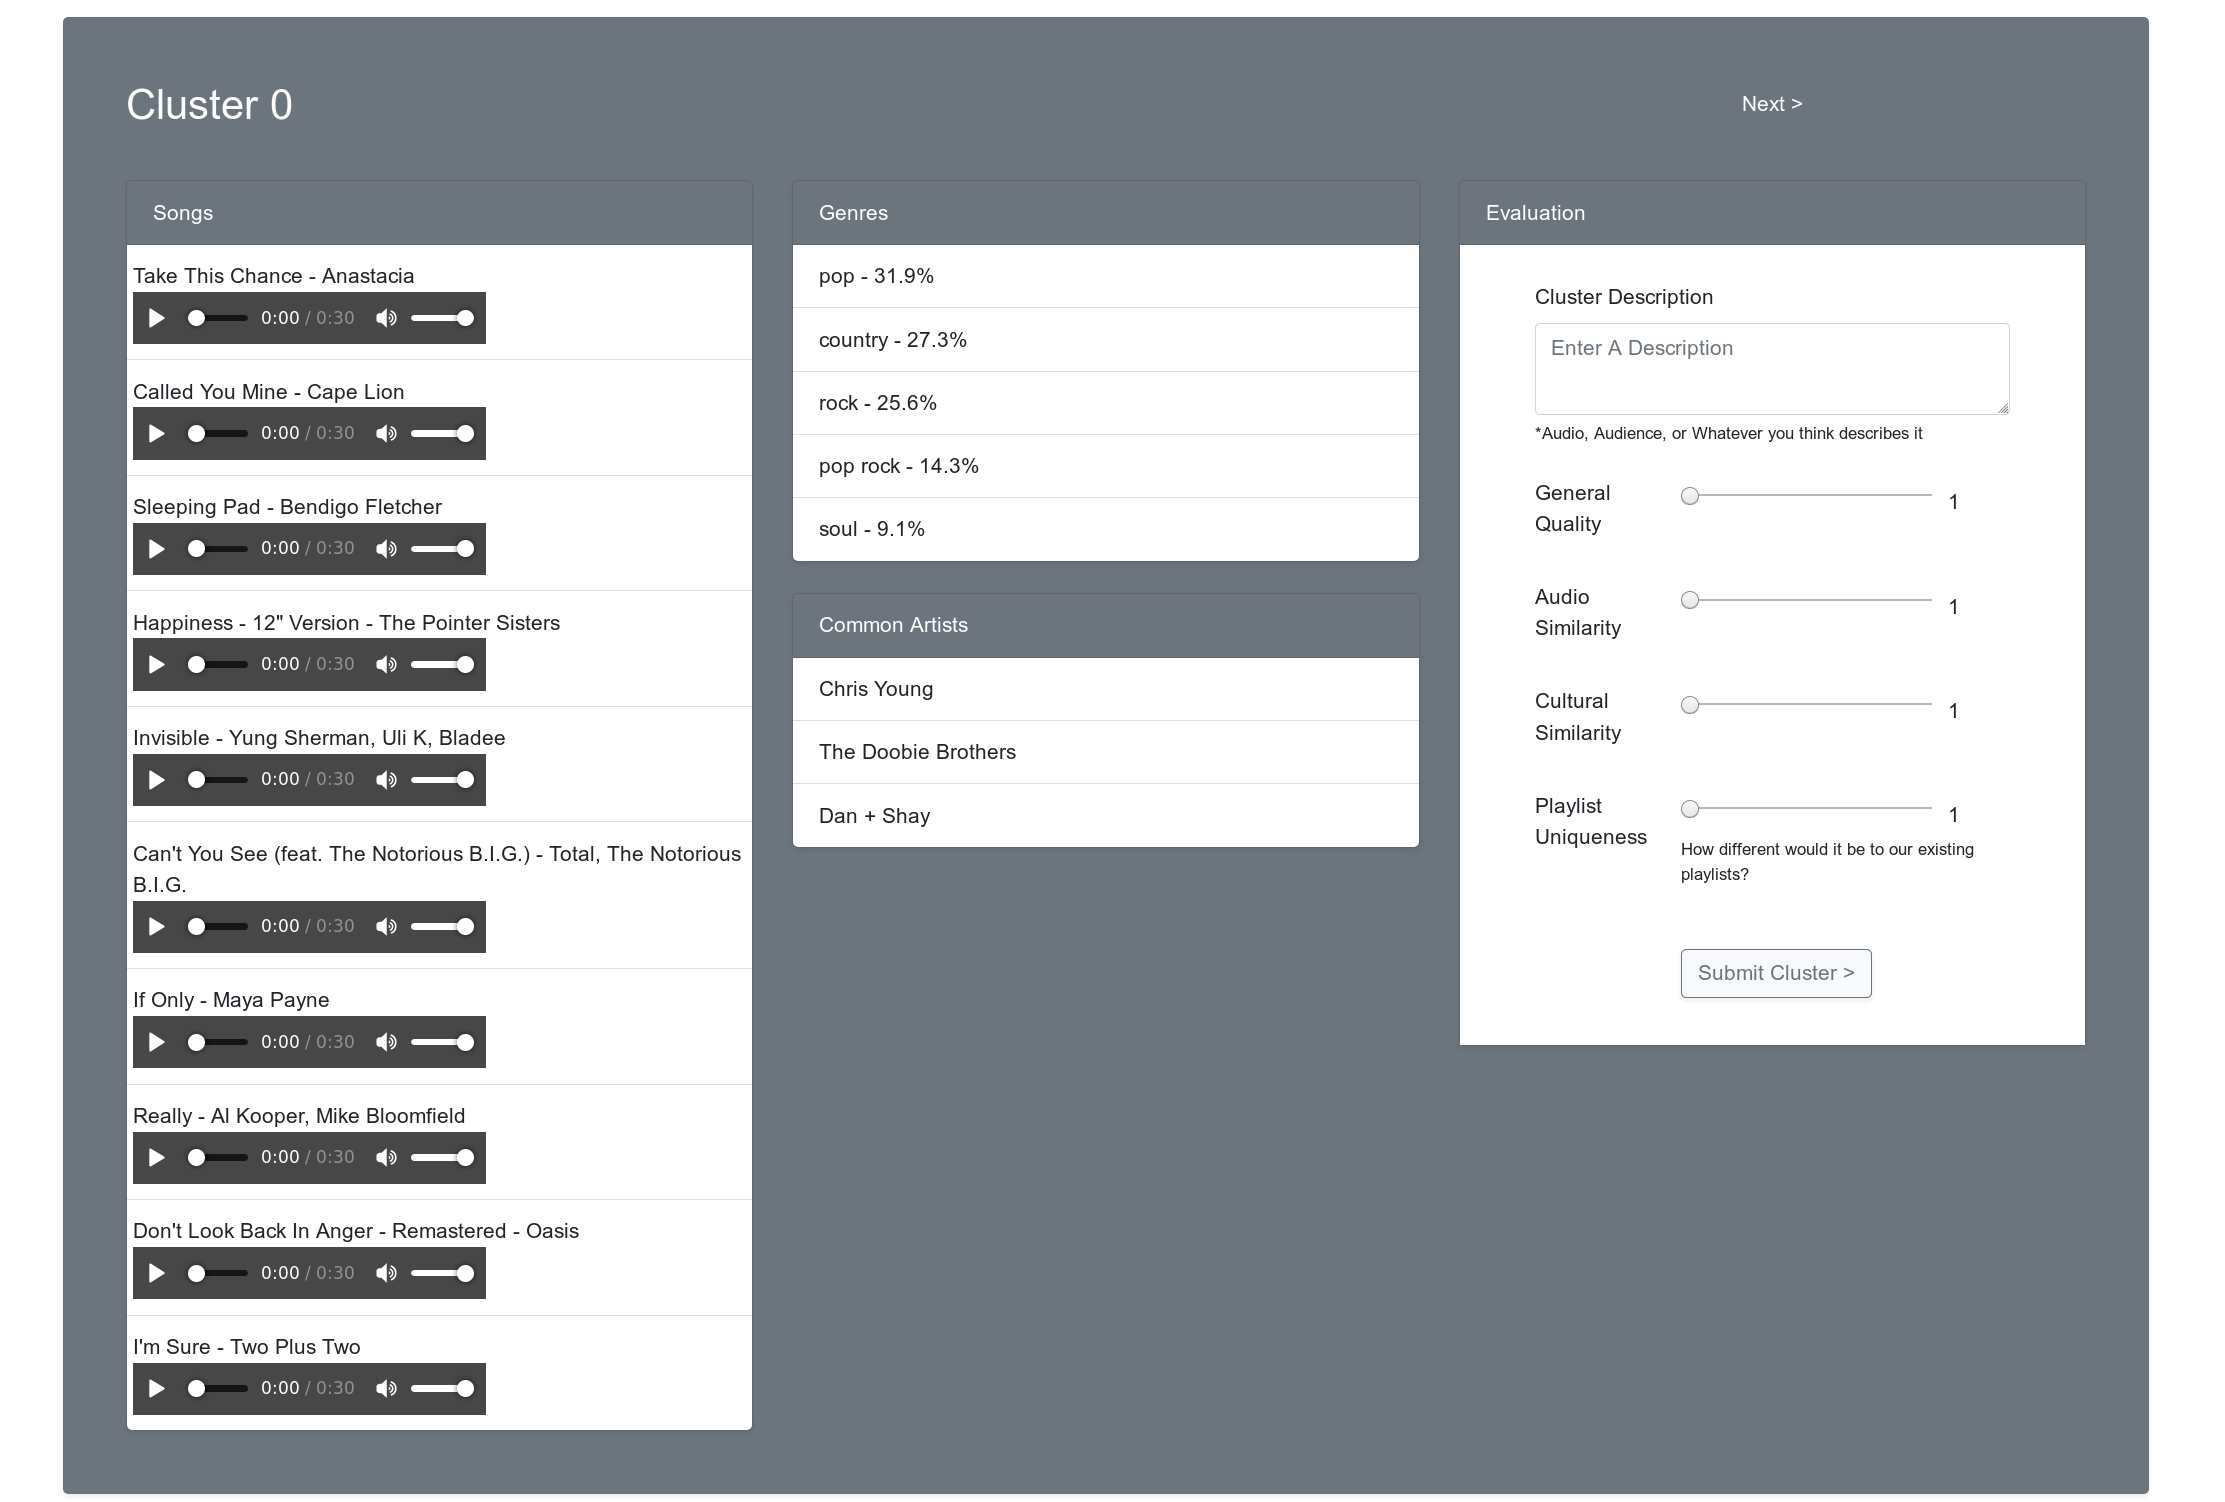
\includegraphics[height=10cm, keepaspectratio]{Website}
    \caption{Screenshot of the evaluation website. \newline
      From the left-hand-side song samples are shown and played. In the middle of the picture, statistics about genres and common artists are shown. On the right-hand-side of the picture, the evaluation form is situated with a general description text area, and sliders for the rest of the evaluation categories.
  }\label{fig:website}
\end{center}
\end{figure}


\end{document}

